\chapter{Strong-production multi-b SUSY search}
\label{chap:strong_prod}


\section{Signal Model}

The simplified models used to optimize this analysis are the two gluino-pair-production models shown in Fig. \ref{fig:strong_diagram}

\begin{figure*}[h]
\centering 
\subfigure[]{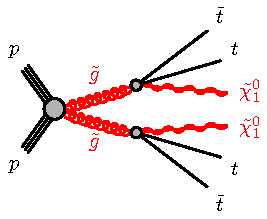
\includegraphics[width=0.35\textwidth]{figures/strong_prod/diagrams/gogo-ttttN1N1.pdf}\label{fig:diagram_Gtt}}
\subfigure[]{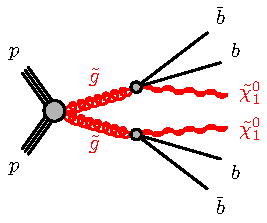
\includegraphics[width=0.35\textwidth]{figures/strong_prod/diagrams/gogo-bbbbN1N1.pdf}\label{fig:diagram_Gbb}}
\caption{The simplified models used for the optimization of the analysis. \subref{fig:diagram_Gtt} Gtt model. \subref{fig:diagram_Gbb} Gbb model.
}\label{fig:strong_diagram}
\end{figure*}



\begin{figure*}[h]
\centering 
\subfigure[]{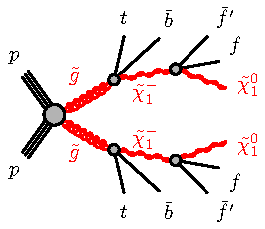
\includegraphics[width=0.35\textwidth]{figures/strong_prod/diagrams/gogo-tbfftbffN1N1.pdf}\label{fig:diagram_strong_tbtb}}
\subfigure[]{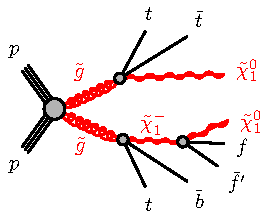
\includegraphics[width=0.35\textwidth]{figures/strong_prod/diagrams/gogo-tttbffN1N1.pdf}\label{fig:diagram_strong_tttb}}\\
\subfigure[]{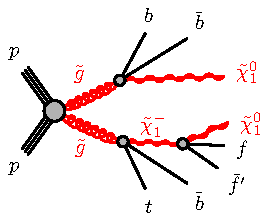
\includegraphics[width=0.35\textwidth]{figures/strong_prod/diagrams/gogo-bbtbffN1N1.pdf}\label{fig:diagram_strong_bbtb}}
\subfigure[]{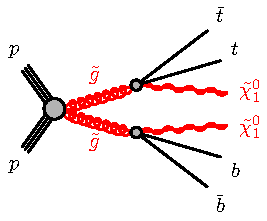
\includegraphics[width=0.35\textwidth]{figures/strong_prod/diagrams/gogo-ttbbN1N1.pdf}\label{fig:diagram_strong_ttbb}}
\caption{Simplified models used in the re-interpretation of the analysis. \subref{fig:diagram_strong_tbtb} Both gluinos have the following decay chain: $\gluino \to t \bar{b} \chinoonem$ with $\chinoonem \to f\bar{f}' \ninoone$. \subref{fig:diagram_strong_tttb} One gluino decays as in \subref{fig:diagram_strong_tbtb} and the other as $\gluino \to t\bar{t}\ninoone$. \subref{fig:diagram_strong_bbtb} One gluino decays as in \subref{fig:diagram_strong_tbtb} and the other as $\gluino \to b\bar{b}\ninoone$. \subref{fig:diagram_strong_ttbb} One gluino decays as $\gluino \to t\bar{t}\ninoone$ and the other as $\gluino \to b\bar{b}\ninoone$.  %The charge conjugate processes are implied.
%The fermions originating from the $\chinoonepm$ decay are typically soft because the mass difference  between the $\chinoonepm$ and the $\ninoone$ is fixed to 2 GeV. 
}\label{fig:strong_diagram_br}
\end{figure*}


\section{Previous Limits}

\section{Analysis Variables}


\section{Pre-fit Data-MC}


\section{Discovery Signal Regions}


\section{Exclusion Signal Regions}

\section{Systematic Uncertainties}

\section{Results}


\section{Interpretation}

\subsection{Model-independent Limits}

\begin{table}[t]
        \centering
        \caption{The $p_0$-values and $Z$ (the number of equivalent Gaussian standard deviations), 
        	the 95$\%$ CL upper limits on the visible cross-section
                ($\sigma^{95}_\mathrm{vis}$),
                and the observed and
                expected 95$\%$ CL upper limits on the number of BSM events ($S_{\textrm
                obs}^{95}$ and $S_{\textrm exp}^{95}$). The maximum
              allowed $p_0$-value
              is truncated at 0.5.}
        \label{mod-ind-lim}
        \small
        \begin{tabular*}{0.6\textwidth}{@{\extracolsep{\fill}}lcccc}
                \noalign{\smallskip}\toprule\noalign{\smallskip}
                Signal channel         & $p_0$ (Z)            & $\sigma^{95}_\mathrm{vis}$ [fb]  &  $S_{\textrm obs}^{95}$  & $S_{\textrm exp}^{95}$   \\
                \noalign{\smallskip}\midrule \noalign{\smallskip}
                SR-Gtt-1L-B & $ 0.50~(0.00) $ &  $0.08$ &  $3.0$ & $ { 3.0 }^{ +1.0 }_{ -0.0 }$ \\[1mm]
                SR-Gtt-1L-M & $ 0.34~(0.42)$ &  $0.11$ &  $3.9$ & $ { 3.6 }^{ +1.1 }_{ -0.4 }$ \\[1mm]
                SR-Gtt-1L-C & $ 0.50~(0.00)$ &  $0.13$ &  $4.8$ & $ { 4.7 }^{ +1.8 }_{ -0.9 }$ \\[1mm]
                \noalign{\smallskip}\midrule \noalign{\smallskip}
                SR-Gtt-0L-B & $ 0.32~(0.48)$ & $0.13$ &  $4.8$ & $ { 4.1 }^{ +1.7 }_{ -0.6 }$  \\[1mm]
                SR-Gtt-0L-M & $ 0.25~(0.69)$ &  $0.21$ &  $7.5$ & $ { 6.0 }^{ +2.3 }_{ -1.4 }$ \\[1mm]
                SR-Gtt-0L-C & $ 0.50~(0.00)$ &  $0.39$ &  $14.0$ & $ { 17.8 }^{ +6.6 }_{ -4.5 }$ \\[1mm] %%to be updated
                \noalign{\smallskip}\midrule\noalign{\smallskip}
                SR-Gbb-B & $ 0.50~(0.00) $ &  $0.13$ &  $4.6$ & $ { 4.6 }^{ +1.7 }_{ -1.0 }$  \\[1mm]
                SR-Gbb-M & $ 0.50~(0.00) $ & $0.12$ &  $4.4$ & $ { 5.0 }^{ +1.9 }_{ -1.1 }$ \\[1mm]
                SR-Gbb-C & $ 0.50~(0.00) $ &  $0.18$ &  $6.6$ & $ { 6.9 }^{ +2.7 }_{ -1.8 }$ \\[1mm]
                SR-Gbb-VC & $ 0.50~(0.00) $ &  $0.08$ &  $3.0$ & $ { 4.6 }^{ +2.0 }_{ -1.3 }$\\
                \noalign{\smallskip}\midrule\noalign{\smallskip}
        \end{tabular*}
\end{table}

\subsection{Model-dependent Limits}

\begin{figure}[htbp]
	\centering 
	\subfigure[]{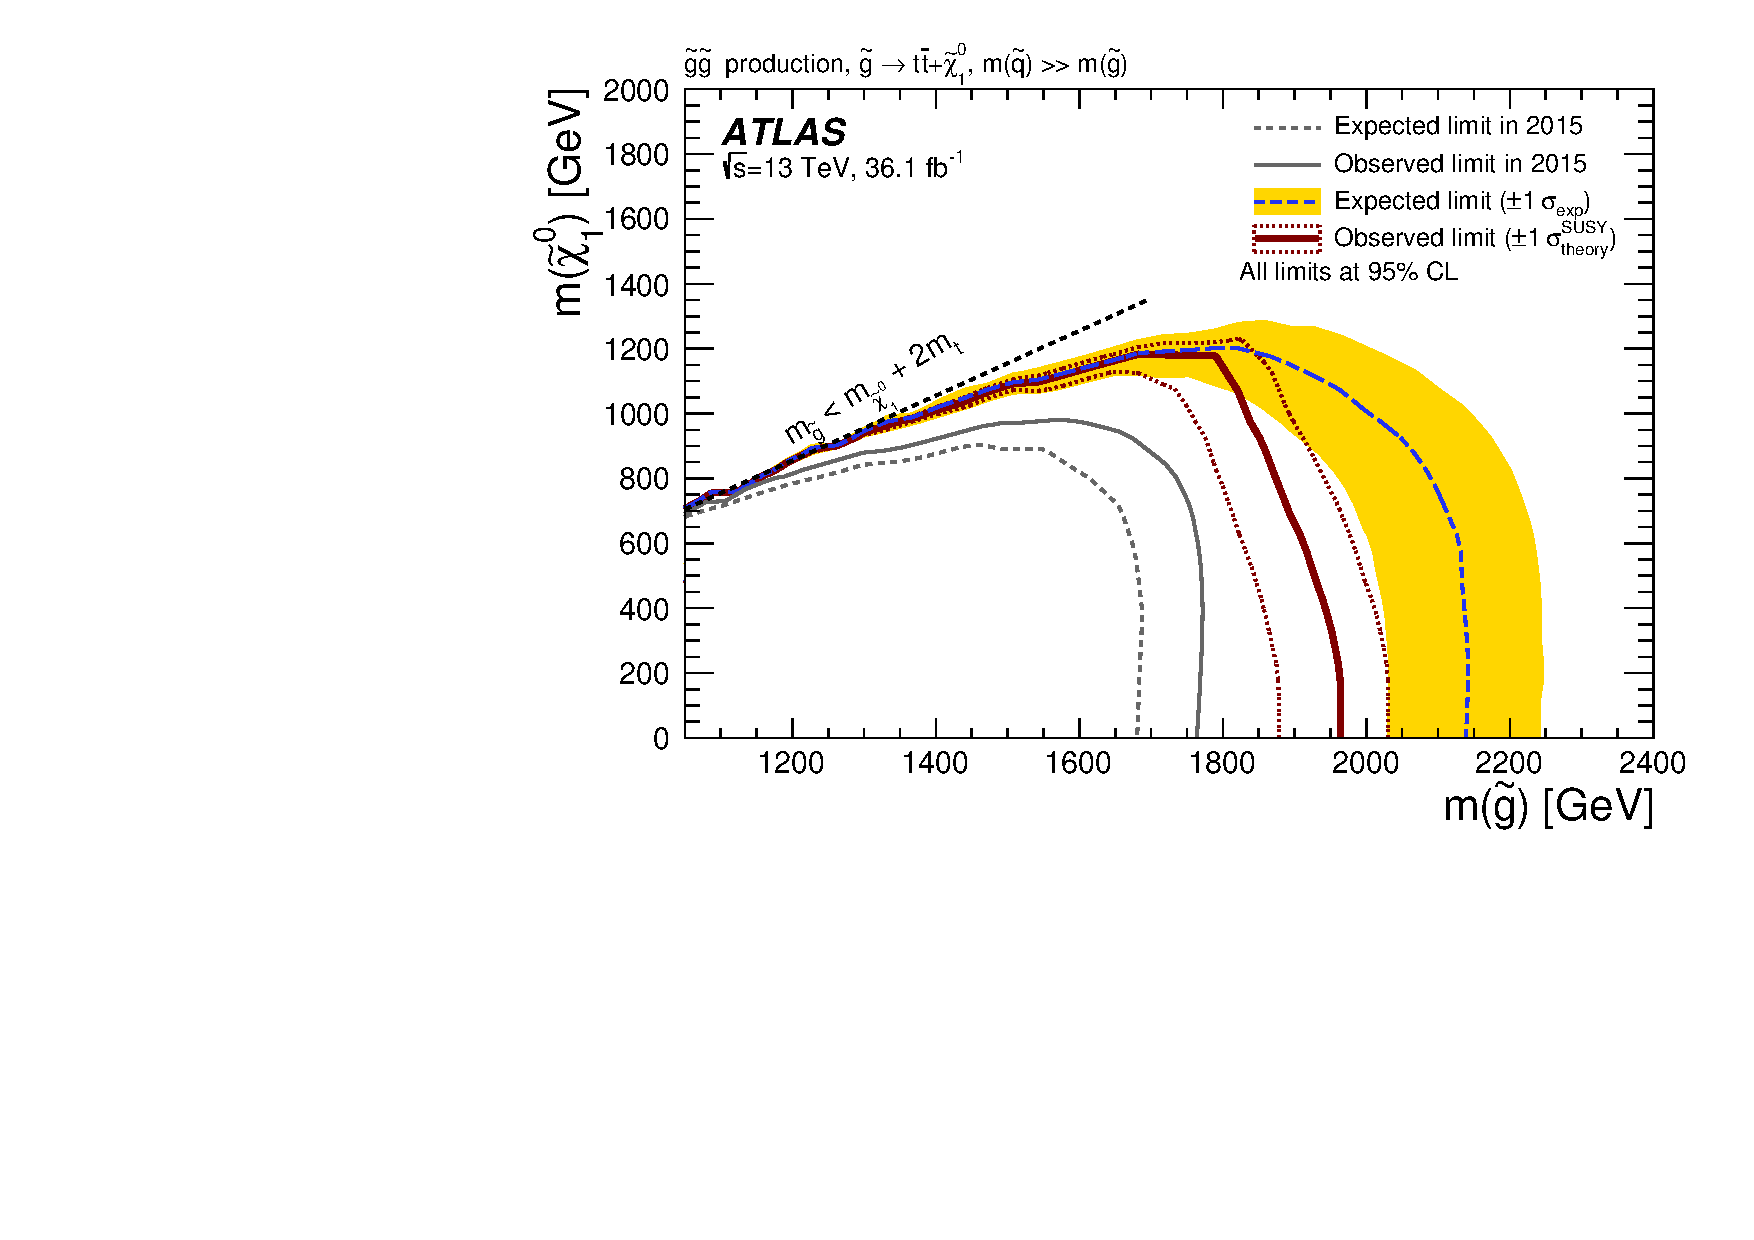
\includegraphics[width=0.65\textwidth]{figures/strong_prod/paper/limits/Limits_Gtt.pdf}\label{fig:limits_Gtt}}
	\subfigure[]{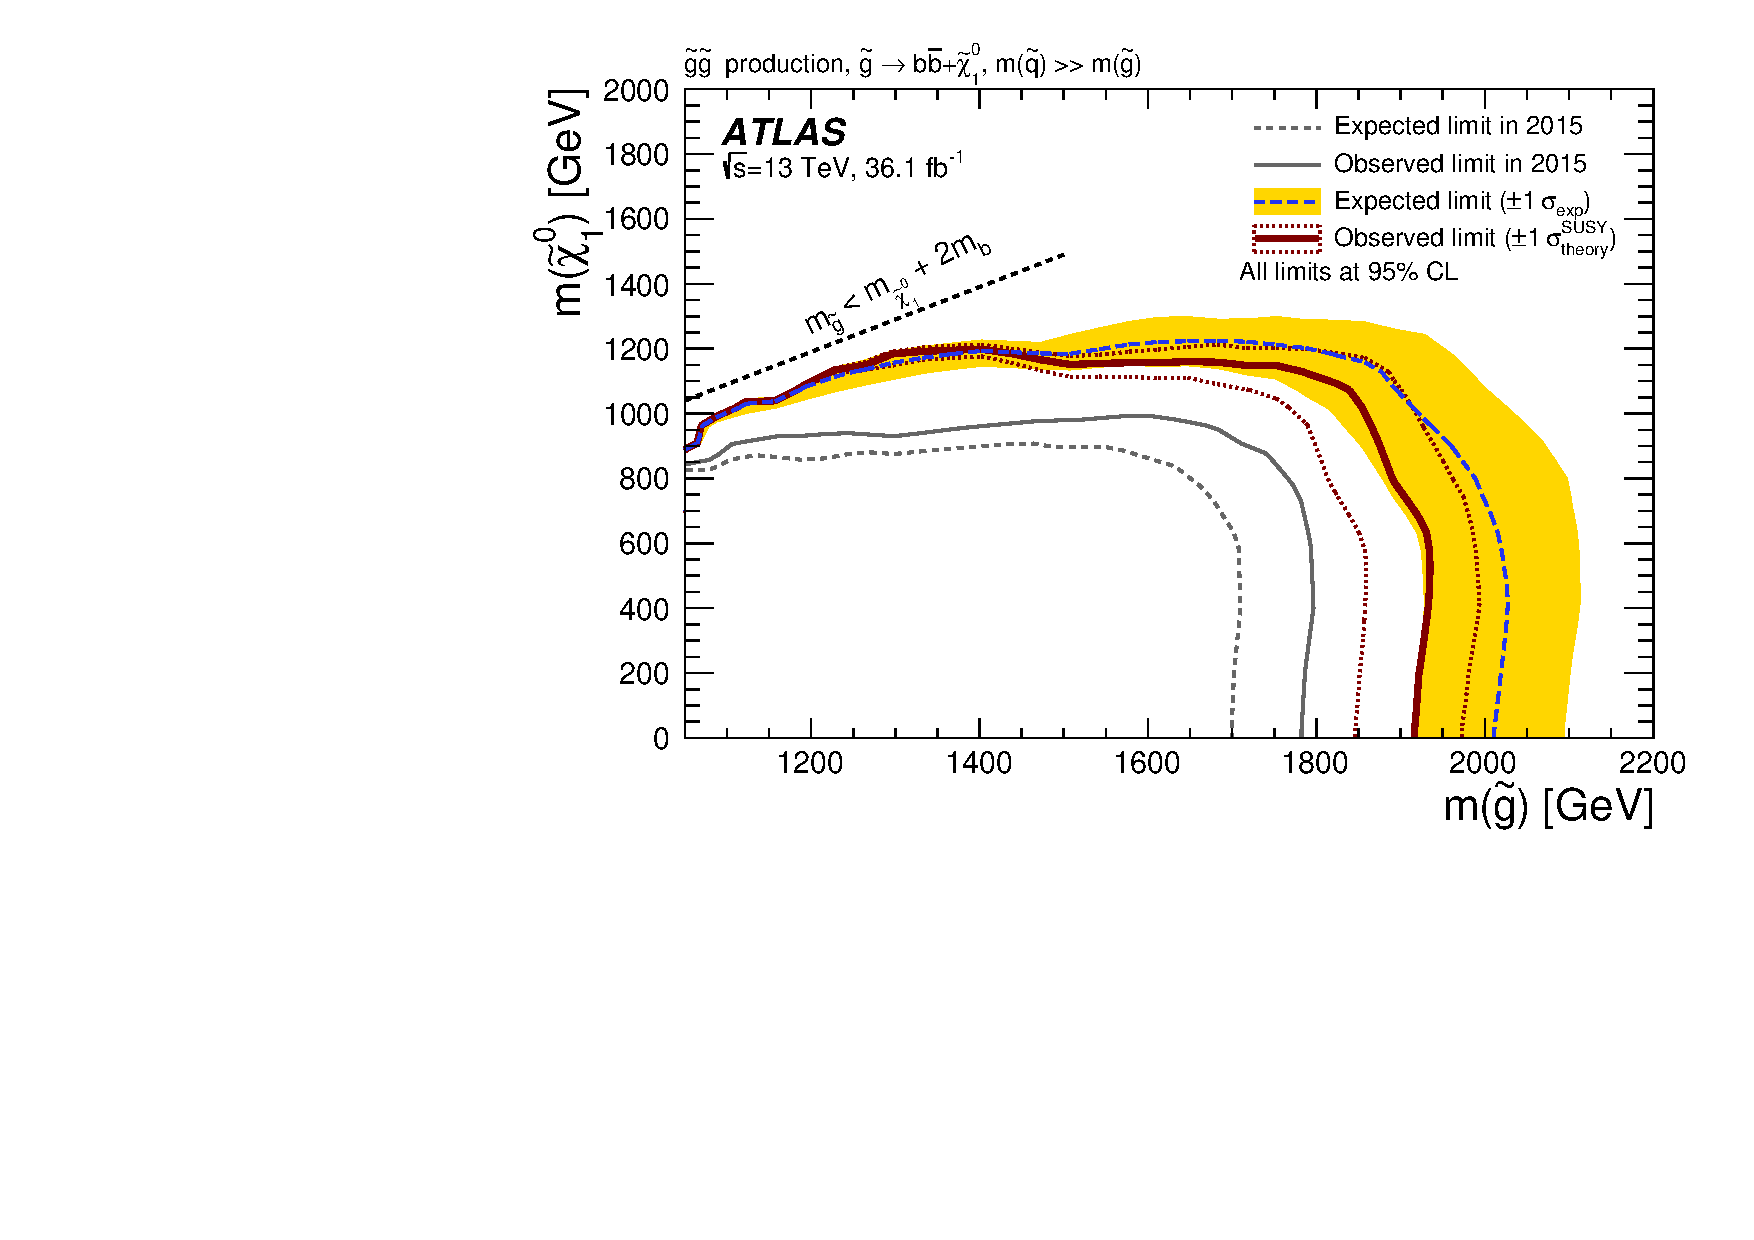
\includegraphics[width=0.65\textwidth]{figures/strong_prod/paper/limits/Limits_Gbb.pdf}\label{fig:limits_Gbb}}
	\caption{Exclusion limits in the $\ninoone$ and $\gluino$ mass plane
  		for the \subref{fig:limits_Gtt} Gtt and  \subref{fig:limits_Gbb} Gbb models obtained
		in the context of the multi-bin analysis. The dashed and solid bold lines
		show the 95\% CL expected and observed limits, respectively. The
  		shaded bands around the expected limits show the
                impact of the
  		experimental and background uncertainties. The dotted
  		lines show the impact on the observed limit of the variation of the
  		nominal signal cross-section by $\pm 1 \sigma$ of its theoretical
  		uncertainty. 
		The 95\%~CL expected and observed limits from the ATLAS search based on 2015 data 
  		\cite{Aad:2016eki} are also shown.}
	\label{fig:limits_GbbGtt}
\end{figure}


\begin{figure}[htbp]
	\centering
	\subfigure[]{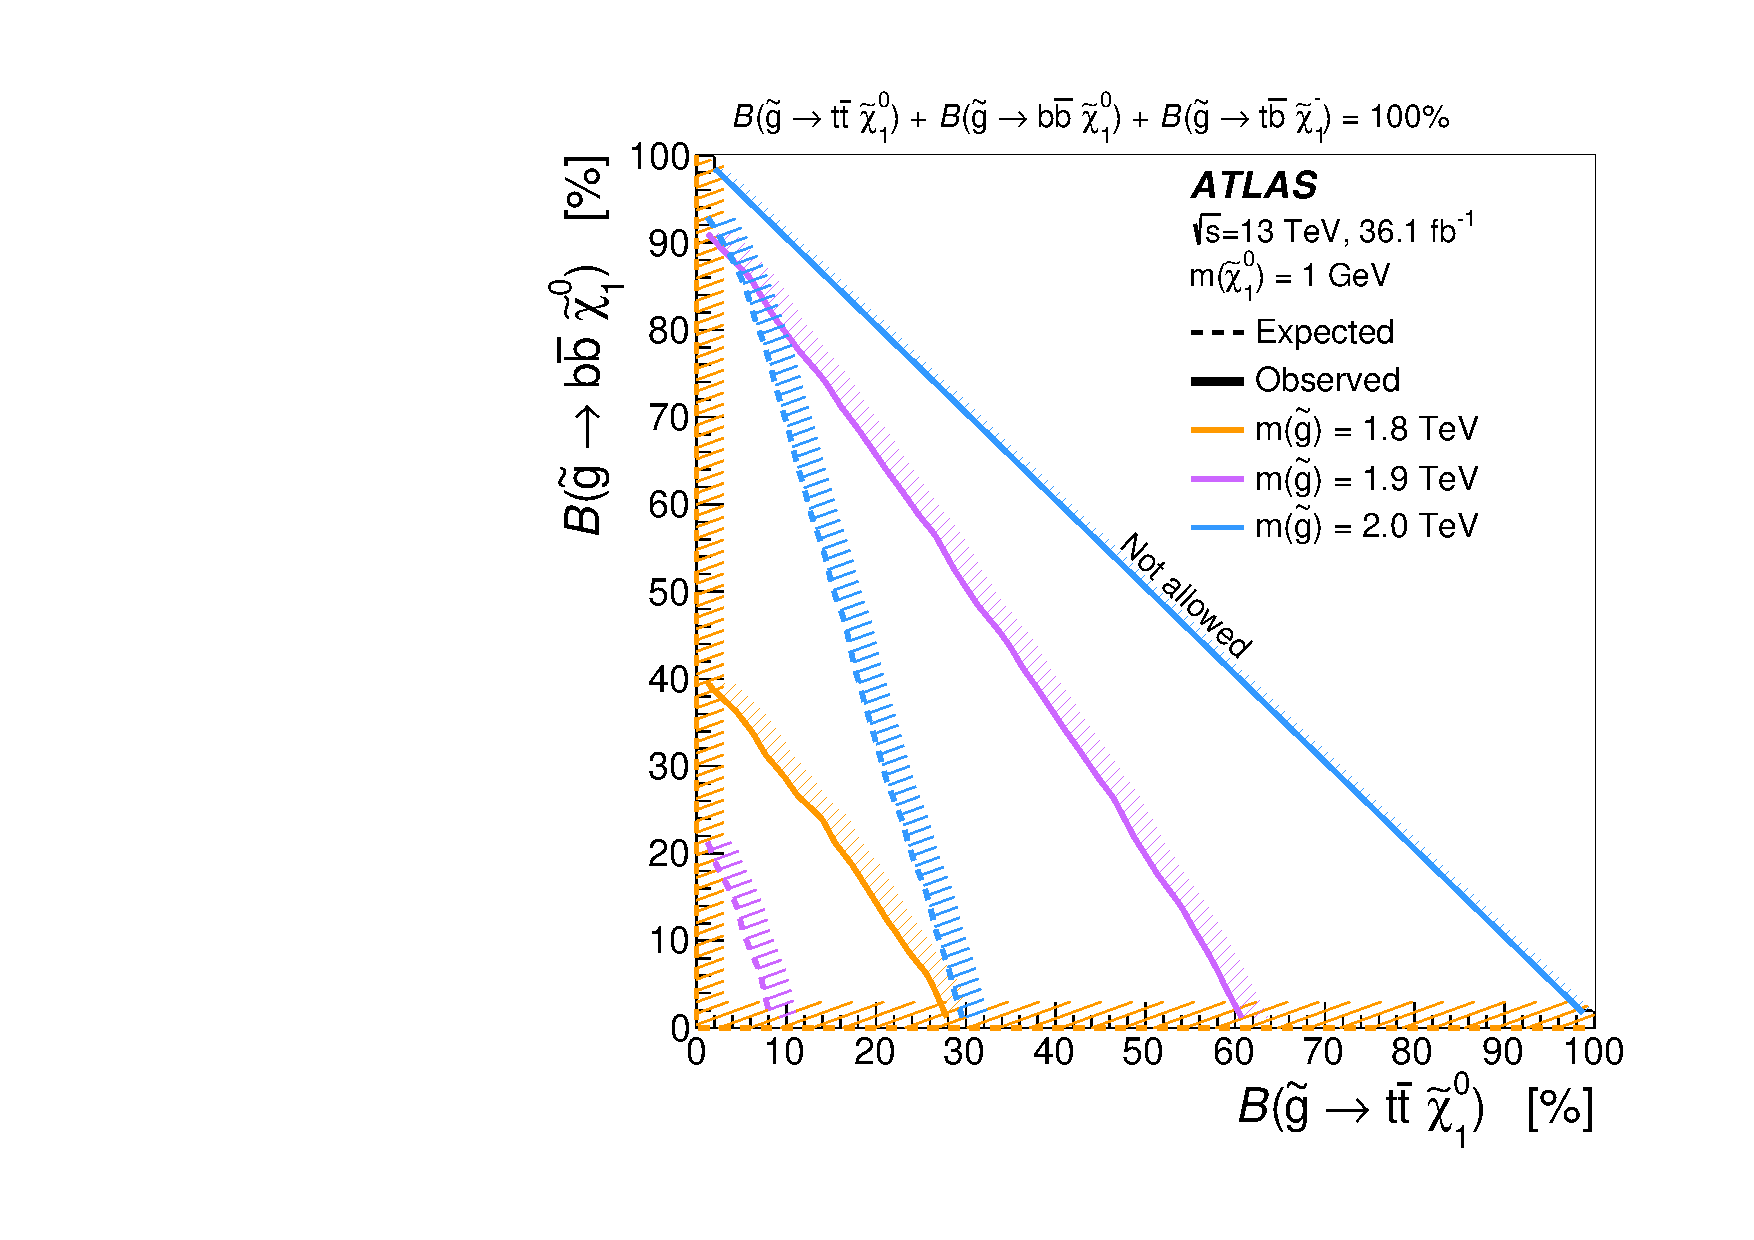
\includegraphics[width=0.65\textwidth]{figures/strong_prod/paper/limits/triangle_UL_massless_neutralino.pdf}\label{fig:limit_br_fixed_neu}}
	\subfigure[]{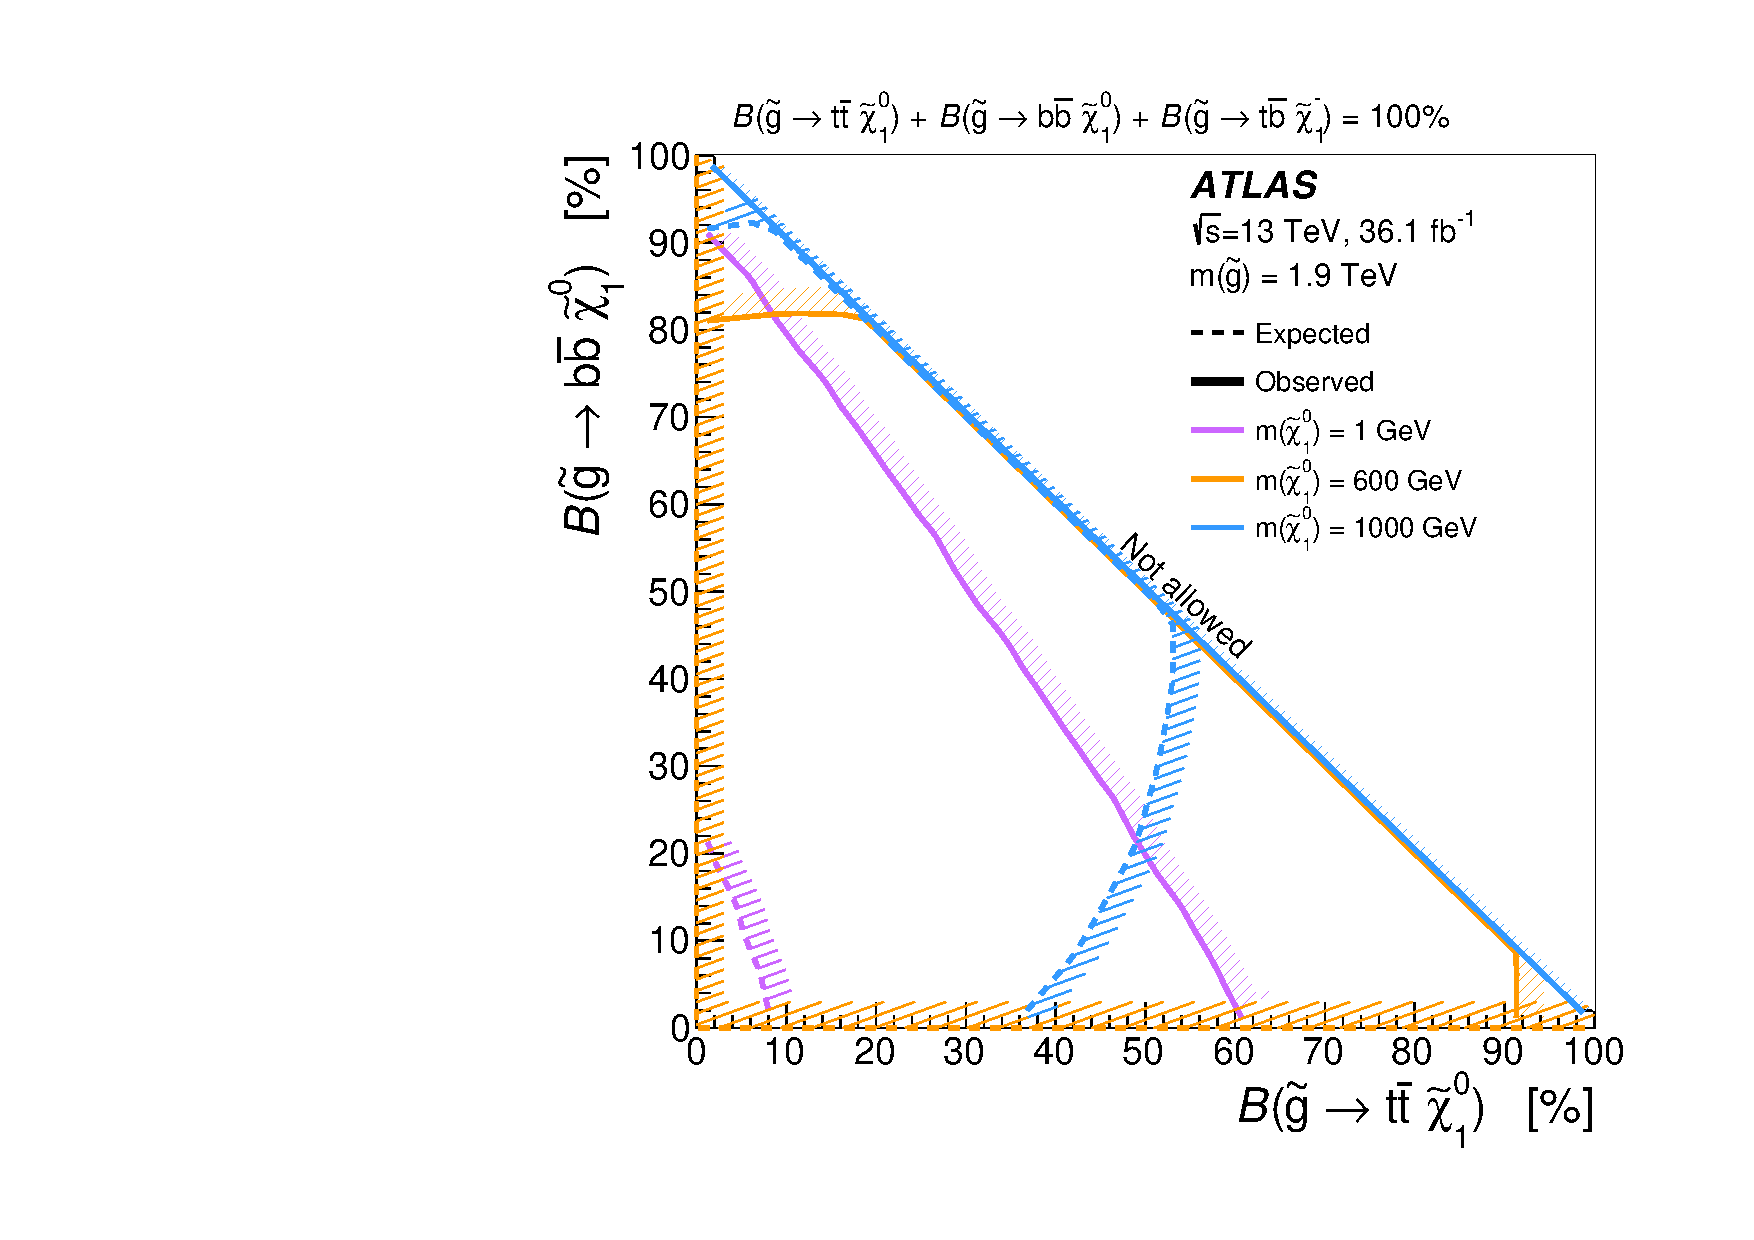
\includegraphics[width=0.65\textwidth]{figures/strong_prod/paper/limits/triangle_UL_1900_gluino.pdf}\label{fig:limit_br_fixed_glu}}
	\caption{Exclusion limits in the $\gluino \to t \bar{t} \ninoone$ and $\gluino \to b \bar{b} \ninoone$
		branching ratio plane assuming \subref{fig:limit_br_fixed_neu} a neutralino mass of 1 GeV and various gluino masses 
		(1.8, 1.9 and 2.0 TeV) and \subref{fig:limit_br_fixed_glu} a gluino mass of 1.9 TeV and three neutralino masses (1, 600 and 1000 GeV). 
		In \subref{fig:limit_br_fixed_neu}, the expected limit for a gluino mass of 1.8 TeV follows the plot axes, meaning that the whole plane is 
		expected to be excluded at 95\% CL.
		The dashed and solid bold lines show the 95\% CL expected and observed limits, respectively. The hashing indicates which side of the line 
		is excluded. The upper right half of the plane is forbidden by the requirement that the sum of branching ratios does not exceed 100\%.}
\end{figure}

\section{Results in the Context of the ATLAS SUSY Group}